\subsection*{Controller C1}

The model of the controller C1 generated is shown in \ref{fig:controller_C1}. The request of packet is generated through \textit{WantIn} action from outside world. C1 controller then communicates to see if a rack space is available by synchronizing with rack controller C5. If rack space is available, the packet is accepted into the system and eventually loaded to one of the elevators, otherwise the packet is rejected.

\begin{figure}[h]
\center
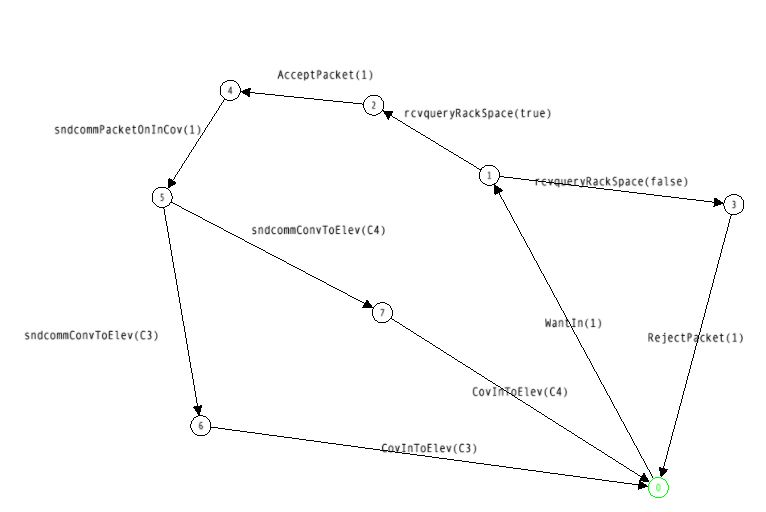
\includegraphics[width=0.7\textwidth]{model_C1}
\caption{Model of controller C1}
\label{fig:controller_C1}
\end{figure}

\subsection*{Controller C2}
The model of the controller C1 generated is shown in \ref{fig:controller_C2}. As mentioned earlier, this controller is responsible for delivering the packet out of the system. With a \textit{WantOut} action, a packet that is requested from outside world is queried with C5(rack) controller on its availability. If available, the packet is brought to the output conveyor by one of the elevators. C2 (output conveyor) controller synchronizes with the elevator controller on receiving the packet and eventually delivers it outside the system. If the requested packet is not found, a \textit{PacketNotFound} action and thus an alarm is initiated informing the user.

\begin{figure}[ht]
\center
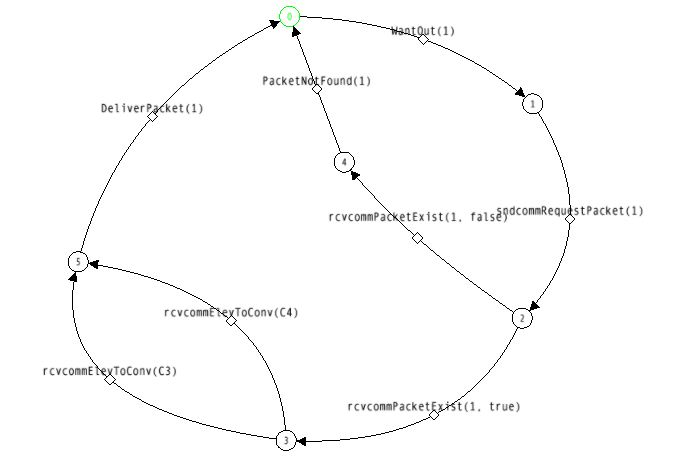
\includegraphics[width=0.7\textwidth]{model_C2}
\caption{Model of controller C2}
\label{fig:controller_C2}
\end{figure}


\subsection*{Controller C3/C4}
Each of the two elevators in the system are controlled independently by their respective elevator controllers, C3 and C4 respectively. The two elevators have similar control characteristics. The model of controller C3 is shown in figure \ref{fig:controller_C3}. This elevator controller synchronizes with C1(input conveyor) controller on packet acceptance, with C5(rack) controller to exchange packets and with C2(output conveyor) controller to deliver the packet out of the system. This controller has the knowledge of the position of its elevator and where it needs to move at any given time.

\begin{figure}[ht]
\center
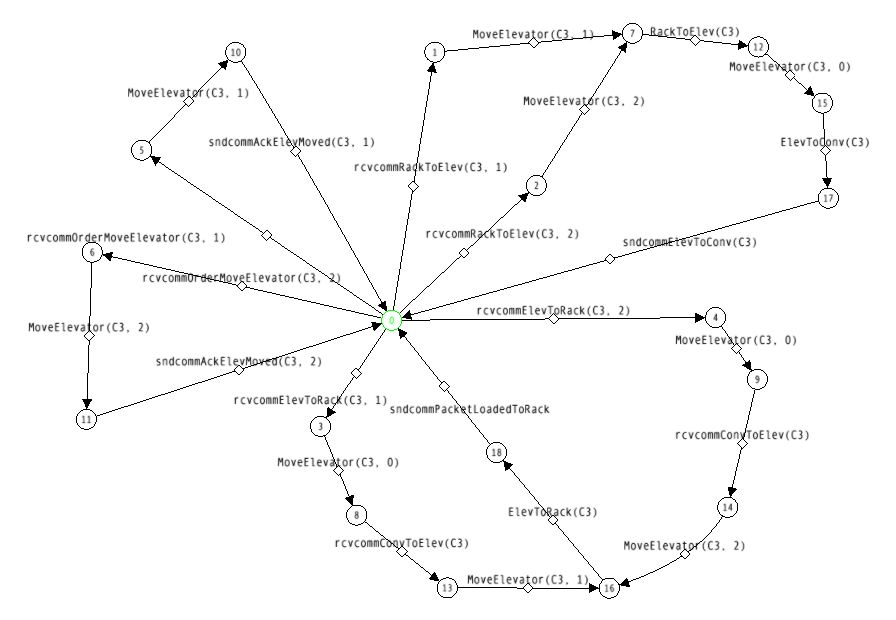
\includegraphics[width=0.7\textwidth]{model_C3}
\caption{Model of controller C3}
\label{fig:controller_C3}
\end{figure}


\subsection*{Controller C5}
The C5 is the rack controller a.k.a master controller which communicates with all the other controllers in the system. It keeps the knowledge of the availability of racks in the system and synchronizes with other controllers and responsible for exchange of packets into and out of the racks. If there is no rack space available and a request is sent to store the packet, it rejects the request.

\begin{figure}[h]
\center
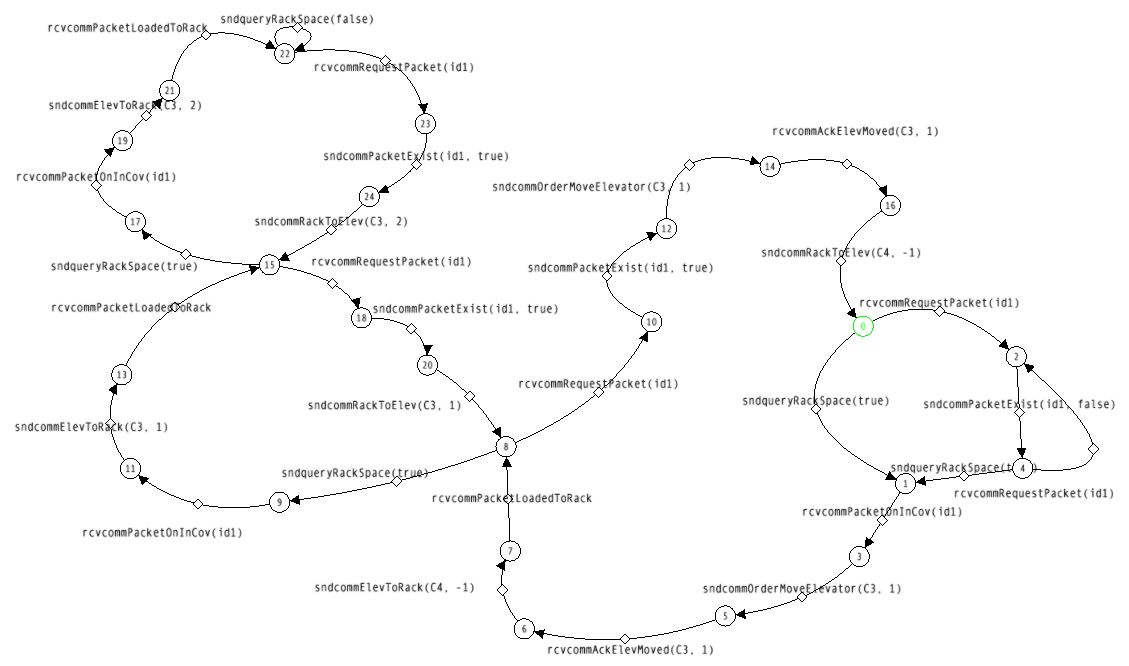
\includegraphics[width=0.7\textwidth]{model_C5}
\caption{Model of controller C5}
\label{fig:controller_C5}
\end{figure}
